\documentclass[zihao=false,fontset=windows]{ctexart}
% ctexart 不接受任意 pt 选项。正文改 {10pt}，方括号里是行距。
\usepackage{scrextend}
\changefontsizes[12pt]{10pt}

\usepackage[a4paper,left=2.35cm,right=2.35cm,top=1.7cm,bottom=1.9cm]{geometry}
\usepackage{xcolor}
\usepackage{graphicx}
\usepackage{amsmath,amssymb}
\usepackage{enumitem}
\usepackage{tabularx}
\usepackage{needspace}
\usepackage{colortbl}
\usepackage{listings}
\usepackage{hyperref}
\usepackage[most]{tcolorbox}

\definecolor{feishuText}{RGB}{31,35,41}
\definecolor{feishuBlue}{RGB}{36,91,219}
\definecolor{feishuRed}{RGB}{216,57,49}
\definecolor{feishuGray}{RGB}{100,106,115}
\definecolor{feishuGray2}{RGB}{143,149,158}
\definecolor{feishuPinkBg}{RGB}{251,191,188}
\definecolor{quoteBar}{RGB}{51,112,255}
\definecolor{codebg}{RGB}{245,246,247}
\definecolor{codeborder}{RGB}{222,224,227}
\definecolor{inlinebg}{RGB}{242,243,245}
\definecolor{callRed}{RGB}{253,226,226}
\definecolor{callOrange}{RGB}{255,245,235}
\definecolor{callYellow}{RGB}{254,255,240}
\definecolor{callGreen}{RGB}{240,251,239}
\definecolor{callBlue}{RGB}{240,244,255}
\definecolor{callRedSoft}{RGB}{254,241,241}
\definecolor{callSun}{RGB}{255,255,204}
\definecolor{tableHead}{RGB}{242,243,245}
\definecolor{tableRule}{RGB}{222,224,227}
\definecolor{codeText}{RGB}{31,35,41}
\definecolor{codeKeyword}{RGB}{0,0,255}
\definecolor{codeComment}{RGB}{0,128,0}
\definecolor{codeString}{RGB}{163,21,21}

\setmainfont{Times New Roman}
\setCJKmainfont{Microsoft YaHei}[AutoFakeBold=2.2]
\setCJKsansfont{Microsoft YaHei}[AutoFakeBold=2.2]
\setCJKmonofont{Microsoft YaHei}[AutoFakeBold=2.2]
\setmonofont{Consolas}
\newfontfamily\emojifont{Segoe UI Emoji}

\hypersetup{
  colorlinks=true,
  urlcolor=feishuBlue,
  linkcolor=feishuBlue,
  unicode=true,
  pdftitle={DeepSeek VL}
}

\setlength{\parindent}{0pt}
\setlength{\parskip}{0.42em}
\setlength{\fboxsep}{1.5pt}
\setlength{\emergencystretch}{3em}
\linespread{1.28}
\color{feishuText}
\arrayrulecolor{tableRule}
\urlstyle{same}

\setlist[enumerate]{label=\textcolor{feishuBlue}{\arabic*.}, leftmargin=1.7em, itemsep=0.22em, topsep=0.28em, parsep=0.08em, partopsep=0pt}
\setlist[itemize,1]{label=\textcolor{feishuBlue}{\textbullet}, leftmargin=1.35em, itemsep=0.18em, topsep=0.25em, parsep=0.06em, partopsep=0pt}
\setlist[itemize,2]{label=\textcolor{feishuBlue}{◦}, leftmargin=1.45em, itemsep=0.12em, topsep=0.15em}
\setlist[itemize,3]{label=\textcolor{feishuBlue}{\rule[0.18em]{0.38em}{0.38em}}, leftmargin=1.55em, itemsep=0.1em, topsep=0.12em}

\newcommand{\feiEmoji}[1]{{\emojifont #1}}
\newcommand{\incode}[1]{\colorbox{inlinebg}{\ttfamily\small #1}}
\newcommand{\bigmath}[1]{%
  \begin{center}\large$\displaystyle #1$\end{center}%
}

\lstset{
  language=Python,
  basicstyle=\ttfamily\footnotesize\color{codeText},
  keywordstyle=\color{codeKeyword},
  commentstyle=\color{codeComment},
  stringstyle=\color{codeString},
  showstringspaces=false,
  breaklines=true,
  columns=fullflexible,
  keepspaces=true,
  tabsize=4,
  upquote=true,
  aboveskip=2pt,
  belowskip=0pt,
  xleftmargin=0pt,
  frame=none
}

\tcbset{
  feishubase/.style 2 args={
    enhanced,
    boxrule=0pt,
    arc=8pt,
    left=10pt,
    right=10pt,
    top=7pt,
    bottom=7pt,
    before skip=6pt,
    after skip=6pt,
    colback=#1,
    colframe=#1,
    before upper={\feiEmoji{#2}\hspace{0.45em}\ignorespaces}
  }
}
\newtcolorbox{feishubox}[2]{feishubase={#1}{#2}, breakable}
\newtcolorbox{feishuboxnb}[2]{feishubase={#1}{#2}}

\newtcolorbox{feishuquote}{
  enhanced,
  breakable,
  boxrule=0pt,
  leftrule=3pt,
  arc=0pt,
  colframe=quoteBar,
  colback=white,
  left=8pt,
  right=2pt,
  top=2pt,
  bottom=2pt,
  before skip=4pt,
  after skip=4pt,
  before upper=\color{feishuGray}
}

\newtcolorbox{feishucode}{
  enhanced,
  breakable,
  colback=codebg,
  colframe=codeborder,
  boxrule=0.6pt,
  arc=6pt,
  left=6pt,
  right=6pt,
  top=5pt,
  bottom=4pt,
  before skip=6pt,
  after skip=6pt
}



% Source: https://scnajei2ds6y.feishu.cn/wiki/B2SDwuImjimZ4TksKCpcF7e9nnb
% Code blocks omitted by user request. Equations visually transcribed from rendered page.


\begin{document}
{\zihao{1}\bfseries DeepSeek VL\par}


\begin{feishuquote}

优势：处理高分辨率图像（1024 x 1024），同时保持相对较低的计算开销。\par

\end{feishuquote}

\par\Needspace{8\baselineskip}\vspace{0.95em}\noindent{\zihao{-2}\bfseries \textcolor{feishuBlue}{1.}\hspace{0.45em}训练阶段}\par\vspace{0.28em}

\begin{center}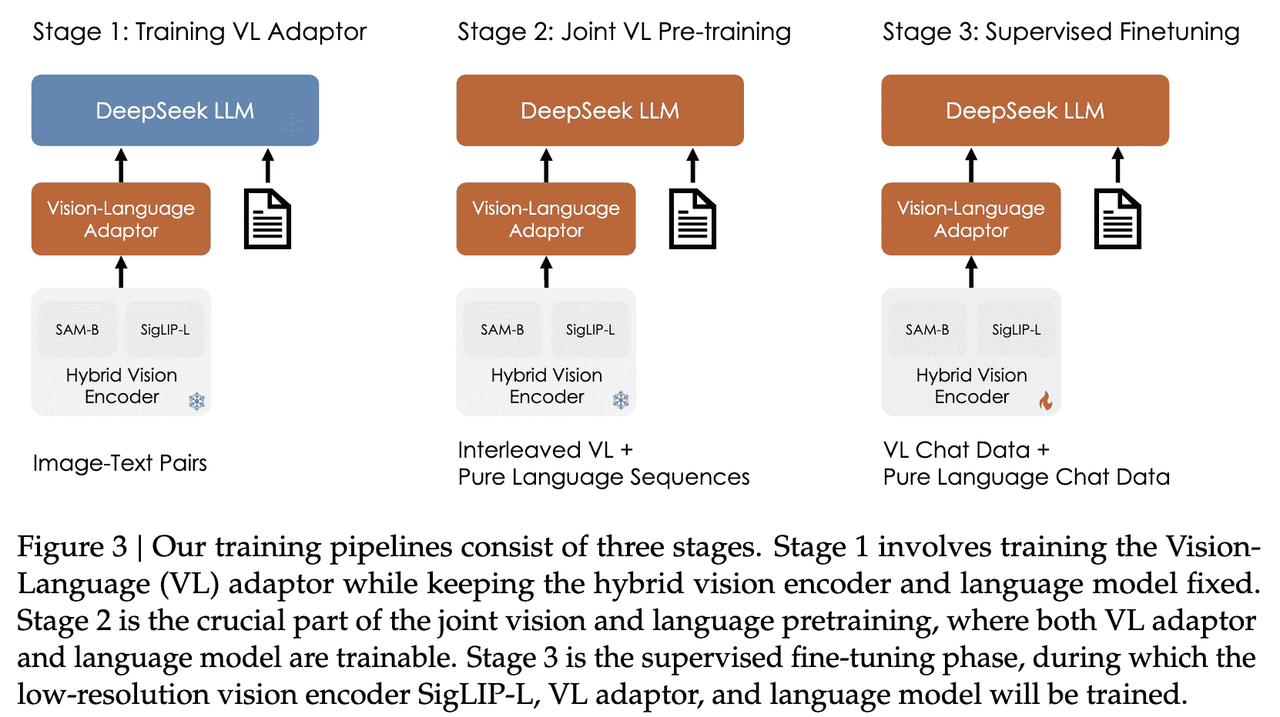
\includegraphics[width=\linewidth,height=0.72\textheight,keepaspectratio]{images/DeepSeek-VL/fig-01.png}\end{center}

\begin{itemize}

\item Step 1: 训练Adaptor，数据为ShareGPT4V（125 万个图文pair），以及250 万个从文档OCR出来的图文pair。

\item Step 2: 放开LLM训练，利用LLM zero-shot能力对齐，以及用纯文本数据保持LLM语言能力，训练数据多模态数据：纯文本数据=7：3。

\item Step 3: 指令微调，SFT。

\end{itemize}

\par\Needspace{8\baselineskip}\vspace{0.95em}\noindent{\zihao{-2}\bfseries \textcolor{feishuBlue}{2.}\hspace{0.45em}模型结构}\par\vspace{0.28em}

参考Fig. 3，采用的是MLLM主流的Vision Encoder（预训练）+Adaptor桥接+LLM的模型结构。\par

\par\Needspace{8\baselineskip}\vspace{0.95em}\noindent{\zihao{3}\bfseries \textcolor{feishuBlue}{2.1}\hspace{0.45em}Hybrid Vision Encoder}\par\vspace{0.28em}

设计了一个Hybrid Vision Encoder，使用两个不同分辨率的ViT:\par

\begin{itemize}

\item SigLIP的ViT接收384*384低分辨率的图像，用来提取粗粒度的图像信息；

\end{itemize}

sigLIP相比与CLIP在loss (CLIP为InfoNCE)上进行了优化：\par

\bigmath{-\frac{1}{|\mathcal B|}\sum_{i=1}^{|\mathcal B|}\sum_{j=1}^{|\mathcal B|}\underbrace{\log\frac{1}{1+e^{z_{ij}(-t\mathbf{x}_i\cdot\mathbf{y}_j+b)}}}_{\mathcal L_{ij}}}

主要优化了两点：1）CLIP由于需要batch的scale，分布式训练时候一次前向需要两次allreduce，sigLIP只需要一次。2）偏置 b 缓解了正负样本不均衡问题。\par

SigLIP的模型结构就是十分标准的ViT，输入为384*384，采用16*16的patch，seq长度为24*24=576，采用1024个kernel，输出为(bs=1) 576*1024\par

\begin{itemize}

\item SAM-B的ViT接收1024*1024的高分辨率图像，用来提取细粒度的图像信息；但是我看论文这个ViT是从MAE任务下pretrain的？

\end{itemize}

\begin{center}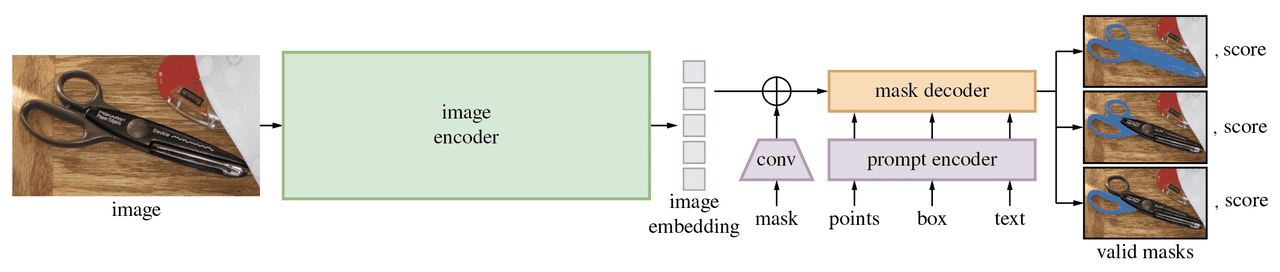
\includegraphics[width=\linewidth,height=0.72\textheight,keepaspectratio]{images/DeepSeek-VL/fig-02.png}\end{center}

高分辨率模型SAM（其实只有SAM的视觉编码器部分）的结构如下图所示，比siglip结构更复杂一些(4)，输出为(bs=1) 576*1024:\par

\begin{center}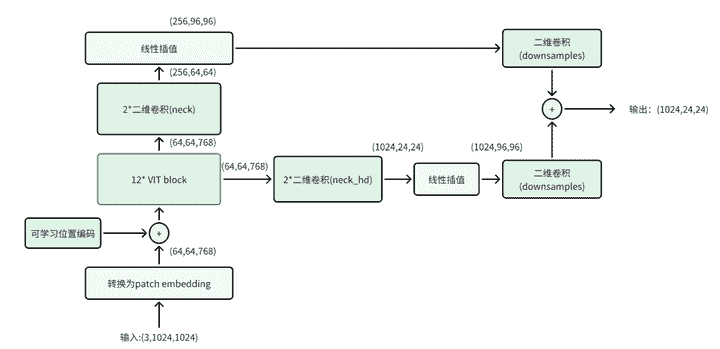
\includegraphics[width=\linewidth,height=0.72\textheight,keepaspectratio]{images/DeepSeek-VL/fig-03.png}\end{center}

\begin{itemize}

\item SigLIP和SAM-VIT特征融合

\end{itemize}

几种可选方式：dim维度拼接、在序列维度拼接、embedding相加、不处理。\par

DeepSeek默认采用不处理，用Adaptor完成融合。\par

\par\Needspace{8\baselineskip}\vspace{0.95em}\noindent{\zihao{3}\bfseries \textcolor{feishuBlue}{2.2}\hspace{0.45em}Adaptor}\par\vspace{0.28em}

分别使用siglip和SAM的VIT结构得到图像的token embedding（维度都为(576,1024)）表示之后，需要使用适配器（由MlpProjector类实现）将图像token embeding映射到和文本token embedding对齐。具体结构如下：\par

\begin{center}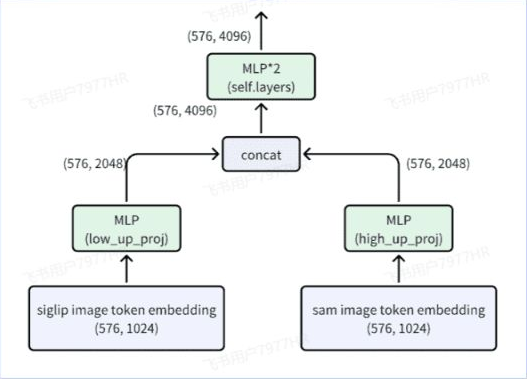
\includegraphics[width=\linewidth,height=0.72\textheight,keepaspectratio]{images/DeepSeek-VL/fig-04.png}\end{center}

\par\Needspace{8\baselineskip}\vspace{0.95em}\noindent{\zihao{3}\bfseries \textcolor{feishuBlue}{2.3}\hspace{0.45em}LLM}\par\vspace{0.28em}

用的是deepseek的语言模型基座。\par

\end{document}